\subsection{近似方案}
\begin{center}
	杨雅晴
\end{center}

在本章前三节中,重点关注的是推导外势作用下单链模型配分函数的精确表达式以及平均性质.大多数情况下,这些表达式并不适合进行精确分析.虽然完整的数值解非常重要,但若能得到一些近似解析表达式(比如配分函数$Q[w]$和密度算子$\rho(\mathbf{r};[w])$的近似解析式)也非常有帮助.这些可用于聚合物流体的多链场理论的分析研究.更重要的,理解单链平均值和算子的渐近行为可以帮助发展多链场理论的有效数值方法.

本节将集中讨论推导配分函数和单链平均值的系统扰动展开的方法.这种渐近方法最直接地应用于Fokker-Planck方程可用的连续链模型.因此,对于连续高斯链和类虫链,可以利用偏微分方程正则摄动和奇异摄动方法的大量文献.在本节中,我们将注意力限制在连续链模型上,并尝试提供一个微扰展开的指南.
\subsubsection{弱非均匀性展开}
当应用的势场$w$具有振幅较弱的不均匀性时,可以得到一个有用的微扰展开式.

为了定义此情形,引入势的体积平均值:
\begin{equation}
w_0\equiv \frac{1}{V} \int w(\mathbf{r})\,\mathrm{d}\mathbf{r}
\end{equation}
并重新定义$w(\mathbf{r})$:
\begin{equation}
w(\mathbf{r})=w_0+\omega(\mathbf{r}) \label{3.113}
\end{equation}
其中,$\omega(\mathbf{r})$用于定义场的非均匀部分.
当非均匀性很弱时,描述振幅特征的小参数$\epsilon_a$ $(|\epsilon_a| \ll 1)$可以从$\omega(\mathbf{r})$中提取出来,即方程(\ref{3.113})改写为:
$$w(\mathbf{r})=w_0+\epsilon_a \omega(\mathbf{r})$$

对于聚合物的连续高斯链模型,Fokker-Planck方程及其初始条件为:
\begin{equation}
\frac{\partial}{\partial s} q(\mathbf{r},s) = \frac{b^2}{6} \bigtriangledown^2 q(\mathbf{r},s) -w_0 q(\mathbf{r},s) -\epsilon_a \omega(\mathbf{r}) q(\mathbf{r},s) \label{3.114}
\end{equation}
\begin{equation}
q(\mathbf{r},0) = 1 \label{3.115}
\end{equation}
其中并不标记$q$关于$w = w_0+\epsilon_a \omega$的函数依赖性.方程(\ref{3.114})的右边中与$w_0$成比例的项可以用以下代换消掉:
\begin{equation}
q(\mathbf{r},s) = e^{-w_0 s} p(\mathbf{r},s) \label{3.116}
\end{equation}
从而得到:
\begin{equation}
\frac{\partial}{\partial s} p(\mathbf{r},s) = \frac{b^2}{6} \bigtriangledown^2 p(\mathbf{r},s) -\epsilon_a \omega(\mathbf{r}) p(\mathbf{r},s) \label{3.117}
\end{equation}
\begin{equation}
p(\mathbf{r},0) = 1 \label{3.118}
\end{equation}

假设$p(\mathbf{r},s)$可以写为以下形式并由此考虑弱非均匀性展开:
\begin{equation}
p(\mathbf{r},s) \sim \sum_{j=o}^{\infty} {\epsilon_a}^j p^{(j)} (\mathbf{r},s) \label{3.119}
\end{equation}
其中$p^{(j)} (\mathbf{r},s)$与$\epsilon_a$无关.方程(\ref{3.119})中我们用$\sim$表示渐近展开.因此,方程(\ref{3.119})中右边的无穷级数既可以收敛也可以发散.即便不收敛,其在截断形式下仍可以在$\epsilon_a$足够小时近似于$p(\mathbf{r},s)$.

通过把方程(\ref{3.119})代入方程(\ref{3.117})-(\ref{3.118})计算$p^{(j)}$,并按照$\epsilon_a$的阶数对应计算项.
$$\frac{\partial}{\partial s} (\sum_{j=o}^{\infty} {\epsilon_a}^j p^{(j)} (\mathbf{r},s)) = \frac{b^2}{6} \bigtriangledown^2 (\sum_{j=o}^{\infty} {\epsilon_a}^j p^{(j)} (\mathbf{r},s)) - \omega(\mathbf{r}) (\sum_{j=o}^{\infty} {\epsilon_a}^{j+1} p^{(j)} (\mathbf{r},s))$$

对于首阶$O({\epsilon_a}^0)$,有:
\begin{equation}
\frac{\partial}{\partial s} p^{(0)}(\mathbf{r},s) = \frac{b^2}{6} \bigtriangledown^2 p^{(0)}(\mathbf{r},s)
\end{equation}
\begin{equation}
p^{(0)}(\mathbf{r},0) = 1
\end{equation}
其有平凡解$p^{(0)}(\mathbf{r},s) = 1$.

对于$O(\epsilon_a)$,有:
\begin{equation}
\frac{\partial}{\partial s} p^{(1)}(\mathbf{r},s) = \frac{b^2}{6} \bigtriangledown^2 p^{(1)}(\mathbf{r},s)-\omega(\mathbf{r}) p^{(0)}(\mathbf{r},s)
\end{equation}
\begin{equation}
p^{(1)}(\mathbf{r},0) = 0
\end{equation}
如果所考虑的系统不是无界的或受受周期性边界条件约束的,那么这个初值问题容易通过空间傅里叶变换来解决.

假设$\omega(\mathbf{r})$的傅里叶变换存在,记为$\hat{\omega}(\mathbf{k})$.
由$p^{(0)}(\mathbf{r},s) = 1$,可得
$$\frac{\partial}{\partial s} p^{(1)}(\mathbf{r},s) = \frac{b^2}{6} \bigtriangledown^2 p^{(1)}(\mathbf{r},s)-\omega(\mathbf{r})$$
两边对$p^{(1)}(\mathbf{r},s)$关于$\mathbf{r}$作傅里叶变换,则
$$\frac{\partial}{\partial s}\hat{p}^{(1)}(\mathbf{k},s) = \frac{-k^2 b^2}{6} \hat{p}^{(1)}(\mathbf{k},s)-\hat{\omega}(\mathbf{k})$$
(其中$F(f^{(n)}(x)) = (ik)^n F(f(x))$)
从而$$(\hat{p}^{(1)}(\mathbf{k},s)e^{\frac{k^2 b^2 s}{6}})' = -\hat{\omega}(\mathbf{k}) e^{\frac{k^2 b^2 s}{6}}$$
两边关于s求积分得
$$\hat{p}^{(1)}(\mathbf{k},s)e^{\frac{k^2 b^2 s}{6}}-\hat{p}^{(1)}(\mathbf{k},0) = -\hat{\omega}(\mathbf{k}) \int_{0}^{s} e^{\frac{k^2 b^2 t}{6}}\, \mathrm{d}t$$
又$\hat{p}^{(1)} (\mathbf{k},0) = 0$,所以
$$\hat{p}^{(1)}(\mathbf{k},s) = -\frac{6}{k^2 b^2} (1-e^{-\frac{k^2 b^2 s}{6}}) \hat{\omega}(\mathbf{k})$$
将上式记为:
\begin{equation}
\hat{p}^{(1)}(\mathbf{k},s) = -\hat{h_2}(\mathbf{k},s) \hat{\omega}(\mathbf{k})
\end{equation}
其中
\begin{equation}
\hat{h_2}(\mathbf{k},s) = \frac{6}{k^2 b^2} (1-e^{-\frac{k^2 b^2 s}{6}})
\end{equation}

类似的,对于$O({\epsilon_a}^2)$,有
\begin{equation}
{\hat{p}}^{(2)}(\mathbf{k},s) = \frac{1}{V} \sum_{\mathbf{k}'} \hat{h_3}(\mathbf{k},\mathbf{k}',s)\hat{\omega}(\mathbf{k}-\mathbf{k}')\hat{\omega}(\mathbf{k}')
\end{equation}
其中
\begin{equation}
\hat{h_3}(\mathbf{k},\mathbf{k}',s) = \frac{36}{b^4 k^2 {|\mathbf{k}-\mathbf{k}'|}^2} [1-e^{-\frac{b^2 k^2 s}{6}}-\frac{k^2}{k^2-{|\mathbf{k}-\mathbf{k}'|}^2}(e^{-\frac{b^2 {|\mathbf{k}-\mathbf{k}'|}^2 s}{6}}-e^{-\frac{b^2 k^2 s}{6}})]
\end{equation}

用上述展开式计算配分函数:
\begin{equation}
\begin{aligned}
   Q[w] &= \frac{1}{V} \int q(\mathbf{r},N)\,\mathrm{d}\mathbf{r}\\
&= \frac{1}{V} e^{-w_0 N} \int p(\mathbf{r},N)\,\mathrm{d} \mathbf{r}\\
&= \frac{1}{V} e^{-w_0 N} \int {e^{-i \mathbf{0} \cdot \mathbf{r}} p(\mathbf{r},N)}\,\mathrm{d} \mathbf{r}\\
&\sim \frac{1}{V} e^{-w_0 N} [\hat{p}^{(0)}(\mathbf{0},N)+\epsilon_a \hat{p}^{(1)}(\mathbf{0},N)+\dots]\\
&\sim e^{-w_0 N} [1+\frac{\epsilon_a}{V} \hat{p}^{(1)}(\mathbf{0},N)+\frac{{\epsilon_a}^2}{V} \hat{p}^{(2)}(\mathbf{0},N)+\dots]
\end{aligned}
\end{equation}

上式中的$O(\epsilon_a)$项中,
因$$\hat{p}^{(1)}(\mathbf{0},N) = -\hat{h_2}(\mathbf{0},N) \hat{\omega}(\mathbf{0})$$
又
$$
\begin{aligned}
	\hat{\omega}(\mathbf{0}) &= \int \omega(\mathbf{r})\,\mathrm{d}{\mathbf{r}} \\
	&= \int w(\mathbf{r})\,\mathrm{d}-\int {w_0}(\mathbf{r})\,\mathrm{d} \\
	&= 0
\end{aligned}
$$
所以$O(\epsilon_a)$项为0.
考虑$O({\epsilon_a}^2)$项,记
\begin{equation}
\hat{h_3}(\mathbf{0},\mathbf{k}',N) = \frac{N^2}{2} \hat{g_D}((k' R_g)^2)
\end{equation}
其中${R_g}^2 = \frac{N b^2}{6}$为连续高斯链的无扰动旋转半径,$\hat{g_D}(x)$为Debye函数.
\begin{equation}
\hat{g_D}(x) = \frac{2}{x^2}(e^{-x}+x-1)
\end{equation}
从而,配分函数的弱非均匀性展开可写为以下形式:
\begin{equation}
Q[w] = e^{-w_0 N}[1+\frac{{\epsilon_a}^2 N^2}{2 V^2} \sum_{\mathbf{k}} \hat{g_D}(k^2 {R_g}^2) \omega(\mathbf{k}) \omega(-\mathbf{k})+\dots]
\end{equation}
或将其写为傅里叶逆变换形式:
因
$$
\begin{aligned}
\frac{1}{V} \sum_{\mathbf{k}} \hat{g_D}(k^2 {R_g}^2) \omega(\mathbf{k}) \omega(-\mathbf{k}) &= \frac{1}{V} \sum_{\mathbf{k}} \hat{g_D}(k^2 {R_g}^2) \int \omega(\mathbf{r}) e^{-i \mathbf{k} \cdot \mathbf{r}}\,\mathrm{d} \mathbf{r} \int \omega(\mathbf{r}') e^{-i (-\mathbf{k}) \cdot \mathbf{r}'}\,\mathrm{d} \mathbf{r}' \\ 
 &= \iint \frac{1}{V} \sum_{\mathbf{k}} \hat{g_D}(k^2 {R_g}^2) e^{i\mathbf{k} \cdot (\mathbf{r}'-\mathbf{r})} \omega(\mathbf{r}) \omega(\mathbf{r}')\,\mathrm{d} \mathbf{r} \mathrm{d} \mathbf{r}'\\
 &= \iint g_D(|\mathbf{r}-\mathbf{r}'|) \omega(\mathbf{r}) \omega(\mathbf{r}')\,\mathrm{d} \mathbf{r} \mathrm{d} \mathbf{r}'
\end{aligned}
$$
所以,
\begin{equation}
Q[w] \sim e^{-w_0 N}[1+\frac{{\epsilon_a}^2 N^2}{2 V}\iint g_D(|\mathbf{r}-\mathbf{r}'|) \omega(\mathbf{r}) \omega(\mathbf{r}')\,\mathrm{d} \mathbf{r} \mathrm{d} \mathbf{r}'+\dots] \label{3.132}
\end{equation}
其中
\begin{equation}
\begin{aligned}
g_D(|\mathbf{r}-\mathbf{r}'|) &= \frac{1}{V}\sum_{\mathbf{k}}e^{i\mathbf{k} \cdot (\mathbf{r}-\mathbf{r}')} \hat{g_D}(k^2 {R_g}^2)\\
 &= \frac{1}{(2\pi)^3} \int e^{i\mathbf{k} \cdot (\mathbf{r}-\mathbf{r}')} \hat{g_D}(k^2 {R_g}^2)\,\mathrm{d} \mathbf{k}
\end{aligned}
\label{3.133}
\end{equation}
上式第二个等号仅在极限情况$V \rightarrow \infty $时成立.

通过对方程(\ref{3.132})做变分导,求解段密度算子$\rho(\mathbf{r},[w])$的弱非均匀性展开:
\begin{equation}
\begin{aligned}
\rho(\mathbf{r},[w]) &= -\frac{1}{Q[w]} \frac{\delta Q[w]}{\delta w(\mathbf{r})} \\
                     &\sim -\frac{1}{1+O({\epsilon_a}^2)} [\frac{\delta (e^{-\frac{N}{V} \int w(\mathbf{r})\,\mathrm{d}\mathbf{r}})}{\delta w(\mathbf{r})}(1+O({\epsilon_a}^2)) + e^{-w_0 N}(\frac{\delta (1+O({\epsilon_a}^2)}{\delta w(\mathbf{r})}) ] \\
                     &\sim \rho_0[1-\epsilon_a N \iint g_D(|\mathbf{r}-\mathbf{r}'|) \omega(\mathbf{r}')\,\mathrm{d} \mathbf{r}'+O({\epsilon_a}^2)]
\end{aligned}
\label{3.134}
\end{equation}
其中$\rho_0 = \frac{N}{V}$为单链段密度的体积平均值.

对比方程(\ref{3.132})与(\ref{3.134})可发现密度算子在$O(\epsilon_a \omega)$处有非均匀贡献,而对配分函数的第一个修正为$O({\epsilon_a}^2 {\omega}^2)$.
此外,$Q[w]$正比于$e^{-w_0 N}$,但密度算子$\rho(\mathbf{r};[w])$与$w_0$无关.事实上,在势能的均匀移动下$w(\mathbf{r}) \rightarrow w(\mathbf{r})+w_u$
$Q$和$\rho$有如下变换性质:
\begin{equation}
Q[w+w_u] = e^{-w_u N}Q[w]	,	\rho(\mathbf{r};[w+w_u]) = \rho(\mathbf{r};[w])
\end{equation}

通过对$w(\mathbf{r})$进一步求变分导,可以得到累积密度-密度相关函数(对相关函数)的弱非均匀性展开.
\begin{equation}
\begin{aligned}
{<\hat{\rho}(\mathbf{r})\hat{\rho}(\mathbf{r}')>}_{[w]}-{<\hat{\rho}(\mathbf{r})>}_{[w]}{<\hat{\rho}(\mathbf{r}')>}_{[w]} &= \frac{\delta^2 \ln Q[w]}{\delta w(\mathbf{r}) \delta w(\mathbf{r}')} \\ &= \frac{\delta}{\delta w(\mathbf{r}')}[\frac{1}{Q[w]} \cdot \frac{\delta Q[w]}{\delta w(\mathbf{r})}] \\ &\sim \frac{\delta}{\delta w(\mathbf{r}')}[\rho_0[-1+\epsilon_a N \iint g_D(|\mathbf{r}-\mathbf{r}'|) \omega(\mathbf{r}')\,\mathrm{d} \mathbf{r}'+O({\epsilon_a}^2)]] \\ &\sim \rho_0 N g_D(|\mathbf{r}-\mathbf{r}'|)+O(\epsilon_a)
\end{aligned}
\label{3.136}
\end{equation}

函数$g_D(r)$通过显示配分函数,密度算子以及对相关函数的首项在弱非均匀性展开中起了重要作用.又对相关函数与$w_0$无关,且$O({\epsilon_a}^0)$项由$g_D$决定,所以$g_D(r)$也可以解释为理想连续高斯链的对相关函数.
\begin{figure}[H]
	\centering
	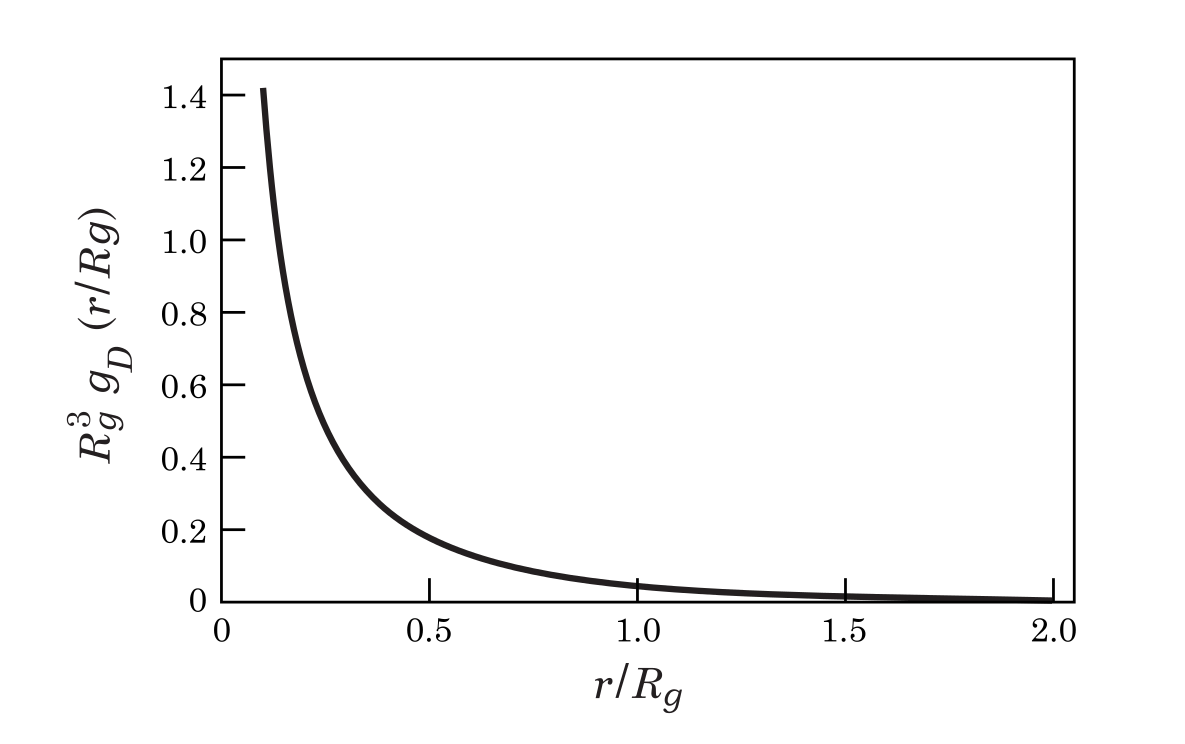
\includegraphics[scale=0.3]{./figures/FIG3-9.png}
	\caption{由(\ref{3.113})定义的Debye函数逆傅里叶变换,并以$\frac{r}{R_g}$为横坐标,以${R_g}^3 g_D(r)$为纵坐标.}
	\label{FIG3.9}
\end{figure}

形如(\ref{FIG3.9}),$\frac{r}{R_g} \ll 1$时,函数以$\frac{1}{r}$的速度代数衰减:
\begin{equation}
g_D(r) \sim \frac{3}{\pi b^2 N r}\label{3.137}
\end{equation}
$r \sim R_g$时,函数单调的指数级的衰减为零:
$$g_D(r) \sim \frac{1}{r} e^{-\frac{\sqrt{3}r}{R_g}}$$

将弱非均匀性展开应用到其他聚合物体系(包括支链聚合物,共聚物)是非常直接的.

例如,在三臂星形均聚物的情况下,臂长相等,即$N_j = N$,
则
\begin{equation}
Q[w] = \frac{1}{V} \int [q(\mathbf{r},N;[w])]^3\,\mathrm{d} \mathbf{r}
\end{equation}
又由(\ref{3.116})和(\ref{3.119})可得
\begin{equation}
Q[w] \sim e^{-3w_0 N} [1+\frac{3 {\epsilon_a}^2 N^2}{2V^2} \sum_{\mathbf{k}} \hat{g_S}(k^2 {R_g}^2)\hat{\omega}(\mathbf{k})\hat{\omega}(-\mathbf{k})+\dots]
\end{equation}
其中${R_g}^2 = \frac{Nb^2}{6}$为星形中一臂的旋转半径,$g_S(x)$为类Debye函数
\begin{equation}
\hat{g_S}(x) = \hat{g_D}(x) + 2[\hat{h_D}(x)]^2
\end{equation}
其中
\begin{equation}
\hat{h_D}(x) = \frac{1}{x} [1-e^{-x}]
\end{equation}
从而密度算子和对相关函数分别为
\begin{equation}
\rho(\mathbf{r};[w]) \sim \rho_0[1-\epsilon_a N \int g_S(|\mathbf{r}-\mathbf{r}') \omega(\mathbf{r}')\,\mathrm{d} \mathbf{r}'+O({\epsilon_a}^2)]
\end{equation}
\begin{equation}
{<\hat{\rho}(\mathbf{r})\hat{\rho}(\mathbf{r}')>}_{[w]} -<\hat{\rho}(\mathbf{r})>_{[w]} <\hat{\rho}(\mathbf{r}')>_{[w]} \sim \rho_0 N g_S(|\mathbf{r}-\mathbf{r}'|)+O(\epsilon_a)
\end{equation}
其中$\rho_0 = \frac{3N}{V}$,且对相关函数表达式与理想星形聚合物的散射函数表达式一致.

弱非均匀性展开也可扩展到类虫链模型:
$$\frac{\partial}{\partial s}q(\mathbf{r},\mathbf{u},s;[w]) = -w(\mathbf{r},\mathbf{u})q(\mathbf{r},\mathbf{u},s;[w])-\mathbf{u} \bigtriangledown_{\mathbf{r}} q(\mathbf{r},\mathbf{u},s;[w])+\frac{1}{2 \lambda}{\bigtriangledown_{\mathbf{u}}}^2 q(\mathbf{r},\mathbf{u},s;[w])$$
$$q(\mathbf{r},\mathbf{u},0;[w]) = 1$$
类似地,考虑摄动展开的$O({\epsilon_a}^j)$项:
\begin{equation}
\frac{\partial}{\partial s}p^{(j)}(\mathbf{r},\mathbf{u},s;[w]) = -\omega(\mathbf{r},\mathbf{u})p^{(j-1)}(\mathbf{r},\mathbf{u},s;[w])-\mathbf{u} \bigtriangledown_{\mathbf{r}}p^{(j)}(\mathbf{r},\mathbf{u},s;[w])+\frac{1}{2 \lambda}{\bigtriangledown_{\mathbf{u}}}^2 p^{(j)}(\mathbf{r},\mathbf{u},s;[w])
\end{equation}
上式本质上相比于理想链Planck方程多了非齐次项$\omega(\mathbf{r},\mathbf{u})p^{(j-1)}(\mathbf{r},\mathbf{u},s;[w])$.
上述方程的空间傅里叶变换原则上可以由球谐展开的连分数表示来求解但仍未有成功计算.

最后,弱非均匀性展开与称为随机相位近似(RPA)的多链系统的近似方案密切相关.这个联系将在5.2.1节展开.

\subsubsection{慢梯度展开}
对于空间中缓慢变化的外势,可以导出另一个重要的渐近展开式.
记
\begin{equation}
w(\mathbf{r}) = \psi_w(\mathbf{r}/\xi_w) \label{3.145}
\end{equation}
其中$\xi_w$为描述$w(\mathbf{r})$空间变化的长度尺度.在$\xi_w$远大于聚合物特征尺寸的情况下,可以推出一个"慢梯度展开".这种渐近展开式最初是用一种与以下方法完全不同的路径积分方法确定的.我们首先在连续高斯链模型中考虑均聚物.

将(\ref{3.145})代入(\ref{3.25})并按下式缩放自变量:
\begin{equation}
t = \frac{s}{N},	\mathbf{x} = \frac{\mathbf{r}}{\xi_w}
\end{equation}
则
\begin{equation}
\frac{\partial}{\partial t}q(\mathbf{x},t) = \epsilon_s {\bigtriangledown_\mathbf{x}}^2 q(\mathbf{x},t)-W(\mathbf{x})q(\mathbf{x},t) \label{3.147}
\end{equation}
其中$W(\mathbf{x}) = N\psi_w(\mathbf{r}/\xi_w)$,
\begin{equation}
\epsilon_s = \frac{N b^2}{6 {\xi_w}^2} = (\frac{R_g}{\xi_w})^2
\end{equation}	
式(\ref{3.147})中$q(\mathbf{x},t;[W])$对$W(\mathbf{x})$的函数依赖性被抑制.且由上述缩放,初始条件(\ref{3.26})为$q(\mathbf{x},0;[W]) = 1$.
在$\xi_w$相比聚合物半径$R_g$很大的条件下,$\epsilon_s$很小,可以作为微扰展开的基础.

慢梯度展开可由下式定义:
\begin{equation}
q(\mathbf{x},t) \sim \sum_{j=0}^{\infty} {\epsilon_s}^j q^{(j)}(\mathbf{x},t) \label{3.149}
\end{equation}
其中$q^{(j)}$与${\epsilon_s}^j$无关.
将式(\ref{3.149})代入(\ref{3.147})以及初始条件,按$\epsilon_s$的阶分出方程的层次结构.从而可得以下结果.

$O({\epsilon_s}^0)$处:
\begin{equation}
\frac{\partial}{\partial t}q^{(0)}(\mathbf{x},t) = -W(\mathbf{x}) q^{(0)}(\mathbf{x},t)
\end{equation}
\begin{equation}
q^{(0)}(\mathbf{x},0) = 1
\end{equation}
解上述方程组:
$$
\begin{aligned}
\frac{\partial q^{(0)}(\mathbf{x},t)}{q^{(0)}(\mathbf{x},t)} &= -W(\mathbf{x})\partial t\\
\partial[\ln q^{(0)}(\mathbf{x},t)] &= -W(\mathbf{x})\partial t\\
\ln q^{(0)}(\mathbf{x},t) - \ln q^{(0)}(\mathbf{x},0) &= -W(\mathbf{x})t\\
q^{(0)}(\mathbf{x},t) &= e^{-W(\mathbf{x})t}
\end{aligned}
$$
即上述方程有精确解:
\begin{equation}
q^{(0)}(\mathbf{x},t) = e^{-W(\mathbf{x})t} \label{3.152}
\end{equation}

$O({\epsilon_s}^1)$处:
\begin{equation}
\frac{\partial}{\partial t}q^{(1)}(\mathbf{x},t) = -W(\mathbf{x}) q^{(1)}(\mathbf{x},t)+{\bigtriangledown_{\mathbf{x}}}^2 q^{(0)}(\mathbf{x},t)
\end{equation}
\begin{equation}
q^{(1)}(\mathbf{x},0) = 0
\end{equation}
解上述方程组:
$$
\begin{aligned}
e^{W(\mathbf{x})t}\frac{\partial}{\partial t}q^{(1)}(\mathbf{x},t)+W(\mathbf{x})e^{W(\mathbf{x})t}q^{(1)}(\mathbf{x},t) &= e^{W(\mathbf{x})} {\bigtriangledown_{\mathbf{x}}}^2 (e^{-W(\mathbf{x})t})\\
&= e^{W(\mathbf{x})} \bigtriangledown_{\mathbf{x}}(-t e^{-W(\mathbf{x})t} \bigtriangledown_{\mathbf{x}} W(\mathbf{x}))\\
&= t^2 e^{-W(\mathbf{x})t} (\bigtriangledown_{\mathbf{x}} W(\mathbf{x}))^2 - t e^{-W(\mathbf{x})t} {\bigtriangledown_{\mathbf{x}}}^2 W(\mathbf{x})\\
&= t^2 (\bigtriangledown_{\mathbf{x}} W(\mathbf{x}))^2-t {\bigtriangledown_{\mathbf{x}}}^2 W(\mathbf{x})\\
{(e^{W(\mathbf{x})t} q^{(1)}(\mathbf{x},t))'}_{about \, t} &= t^2 (\bigtriangledown_{\mathbf{x}} W(\mathbf{x}))^2-t {\bigtriangledown_{\mathbf{x}}}^2 W(\mathbf{x})\\
e^{W(\mathbf{x})t} q^{(1)}(\mathbf{x},t) &= \frac{t^3}{3}|\bigtriangledown_{\mathbf{x}} W(\mathbf{x})|^2 - \frac{t^2}{2} {\bigtriangledown_{\mathbf{x}}}^2 W(\mathbf{x})
\end{aligned}
$$
即上述方程有精确解:
\begin{equation}
q^{(1)}(\mathbf{x},t) = e^{-W(\mathbf{x})t} [\frac{t^3}{3}|\bigtriangledown_{\mathbf{x}} W(\mathbf{x})|^2 - \frac{t^2}{2} {\bigtriangledown_{\mathbf{x}}}^2 W(\mathbf{x})]
\end{equation}

又由(\ref{3.22}),慢梯度展开的配分函数为:
\begin{equation}
\begin{aligned}
Q[W] &= \frac{\xi_w}{V}\int q(\xi_w \mathbf{x},N,\frac{[W]}{N})\,\mathrm{d}(\xi_w \mathbf{x})\\
&= \frac{{\xi_w}^3}{V}\int q(\mathbf{x},1)\,\mathrm{d}\mathbf{x}\\
&\sim \frac{{\xi_w}^3}\int e^{-W(\mathbf{x})}[1+\epsilon_s(\frac{1}{3}|\bigtriangledown_{\mathbf{x}} W(\mathbf{x})|^2-\frac{1}{2}{\bigtriangledown_{\mathbf{x}}}^2 W(\mathbf{x}))+\dots]\,\mathrm{d}\mathbf{x}\\
&\sim \frac{{\xi_w}^3}\int e^{-W(\mathbf{x})}[1-\frac{\epsilon_s}{6}|\bigtriangledown_{\mathbf{x}} W(\mathbf{x})|^2+O({\epsilon_s}^2)]\,\mathrm{d}\mathbf{x}
\end{aligned}
\end{equation}
其中最后一行由分部积分得到(假设边界项可忽略):
$$
\begin{aligned}
\int e^{-W(\mathbf{x})}{\bigtriangledown_{\mathbf{x}}}^2 W(\mathbf{x})\,\mathrm{d}\mathbf{x} &= \int e^{-W(\mathbf{x})}\,\mathrm{d}(\bigtriangledown_{\mathbf{x}} W(\mathbf{x}))\\
 &= -\int \bigtriangledown_{\mathbf{x}} W(\mathbf{x})\,\mathrm{d}(e^{-W(\mathbf{x})})\\
 &= \int e^{-W(\mathbf{x})}(\bigtriangledown_{\mathbf{x}})^2\,\mathrm{d}\mathbf{x}
\end{aligned}
$$

配分函数的表达式在密度算子和对相关函数的展开中起了重要作用.
比如:
\begin{equation}
\begin{aligned}
\rho(\mathbf{x};[W]) &= \frac{\rho_0}{Q[W]}\int_{0}^{1}q(\mathbf{x},1-t)q(\mathbf{x},t)\,\mathrm{d}t\\
&\sim \frac{\rho_0}{Q[W]}\int_{0}^{1}(\sum_{j=0}^{\infty}{\epsilon_s}^j q^{(j)}(\mathbf{x},1-t))(\sum_{j=0}^{\infty}{\epsilon_s}^j q^{(j)}(\mathbf{x},t))\,\mathrm{d}t\\
&\sim \frac{\rho_0}{Q[W]}\int_{0}^{1}q^{(0)}(\mathbf{x},1-t)q^{(0)}(\mathbf{x},t)+\epsilon_s[q^{(0)}(\mathbf{x},1-t)q^{(1)}(\mathbf{x},t)+q^{(1)}(\mathbf{x},1-t)q^{(0)}
(\mathbf{x},t)]\,\mathrm{d}t\\
&\sim \frac{\rho_0 e^{-W(\mathbf{x})}}{Q[W]}[1+\epsilon_s(\frac{1}{6}|\bigtriangledown_{\mathbf{x}}W|^2-\frac{1}{3} {\bigtriangledown_{\mathbf{x}}}^2 W)+\dots]
\end{aligned}
\end{equation}
其中$\rho_0 = \frac{N}{V}$.

对于连续高斯链模型中的任何聚合物体系结构,都可以很容易地推导出类似的慢梯度展开.但这种展开的适用性很有限,是因为与绝大多数不均匀聚合物流体有关的势在远小于$R_g$的尺度上会产生变化.这些快速势场的变化源于中间厚度介于统计段长度$b(\sim 1nm)$与$R_g(\sim 10nm)$之间的界面.在一些特殊情形下,如临界点附近的聚合物共混物界面可以扩大到$R_g$以外.对于类虫链模型来说,慢梯度展开的作用要小得多.

\subsubsection{基态优势}
分析连续连模型的扩散方程的另一个重要方法是利用特征函数展开,其为量子力学中常见的分析方法.

将(\ref{3.25})写为算子形式:
\begin{equation}
\frac{\partial}{\partial s} q(\mathbf{r},s) = \mathcal{L} q(\mathbf{r},s) \label{3.158}
\end{equation}
其中算子为
\begin{equation}
\mathcal{L} = \frac{b^2}{6}\bigtriangledown^2-w(\mathbf{r})
\end{equation}

对实$w(\mathbf{r})$以及合适的边界条件来说,$\mathcal{L}$为自伴的Sturm-Liouville算子,且其有实特征值$\Lambda_k$以及特征函数$\Psi_k (\mathbf{r})$(完备且正交)满足:
\begin{equation}
\mathcal{L} \Psi_k (\mathbf{r}) = -\Lambda_k \Psi_k (\mathbf{r}),	k=0,1,2\dots \infty \label{3.160}
\end{equation}
其中k使得$\Lambda_k$从小到大排序-$\Lambda_0$为最小特征值.

假设$\Psi_k (\mathbf{r})$已归一化,可用下式表示其正交性:
\begin{equation}
\int \Psi_j (\mathbf{r})\Psi_k (\mathbf{r})\,\mathrm{d}\mathbf{r} = \delta_{jk} \label{3.161}
\end{equation}
\begin{equation}
\sum_{k=0}^{\infty}\Psi_k (\mathbf{r}')\Psi_k (\mathbf{r}) = \delta(\mathbf{r}-\mathbf{r}')
\end{equation}
从而方程(\ref{3.158})的解可以被$\mathcal{L}$的特征函数表示:
\begin{equation}
q(\mathbf{r},s) = \sum_{k=0}^{\infty}q_k \Psi_k (\mathbf{r})e^{-s\Lambda_k} \label{3.163}
\end{equation}
系数$q_k$可以由初始条件$q(\mathbf{r},0;[w])=1$以及正交性得到:
由
$$
\begin{aligned}
\int q(\mathbf{r},s)\Psi_k (\mathbf{r})\,\mathrm{d}\mathbf{r} &= \int \Psi_k (\mathbf{r})\sum_{k=0}^{\infty}q_k \Psi_k (\mathbf{r})e^{-s\Lambda_k}\,\mathrm{d}\mathbf{r}\\
&= \int q_k \Psi_k (\mathbf{r}) \Psi_k (\mathbf{r})e^{-s\Lambda_k}
\end{aligned}
$$
所以,
\begin{equation}
q_k = \int q(\mathbf{r},0)\Psi_k (\mathbf{r})\,\mathrm{d}\mathbf{r} = \int \Psi_k (\mathbf{r})\,\mathrm{d}\mathbf{r}
\end{equation}

除此之外,方程(\ref{3.158})的格林函数解有相关的展开:
\begin{equation}
g(\mathbf{r},\mathbf{r}',s) = \sum_{k=0}^{\infty}\Psi_k (\mathbf{r}')\Psi_k (\mathbf{r})e^{-s\Lambda_k} \label{3.165}
\end{equation}

这种特征函数展开式的效用受限于我们在适当边界条件下解特征值问题的能力以及对无穷级数求和的要求.在聚合物物理的大多数实际情况下,我们既找不到特征值和特征函数的解析表达式,也找不到(\ref{3.163})和(\ref{3.165})这样的精确级数和.

由此引出,一个被称为基态优势近似的重要的近似方案,适用于当特征函数展开可以在$k=0$项后截断时.
比如,此近似应用在配分函数:
\begin{equation}
\begin{aligned}
Q[w] &= \frac{1}{V}\int q(\mathbf{r},N)\,\mathrm{d}\mathbf{r}\\
&= \frac{1}{V}\int \sum_{k=0}^{\infty}q_k \Psi_k (\mathbf{r})e^{-N\Lambda_k}\,\mathrm{d}\mathbf{r}\\
&= \frac{1}{V} \sum_{k=0}^{\infty}q_k e^{-N\Lambda_k}\int \Psi_k (\mathbf{r})\,\mathrm{d}\mathbf{r}\\
&= \frac{1}{V} \sum_{k=0}^{\infty}{q_k}^2 e^{-N\Lambda_k}\\
&\sim \frac{{q_0}^2}{V}e^{-N\Lambda_0}
\end{aligned}
\end{equation}
应用于密度算子:
\begin{equation}
\begin{aligned}
q(\mathbf{r};[w]) &= -\frac{\delta \ln Q[w]}{\delta w(\mathbf{r})}\\
&= -\frac{1}{Q[w]} \frac{{q_0}^2}{V} \frac{\delta[e^{-N\Lambda_0}]}{\delta w(\mathbf{r})}\\
&\sim \frac{N {q_0}^2}{V Q[w]}e^{-N\Lambda_0}(\frac{\delta \Lambda_0}{\delta w(\mathbf{r})})\\
&\sim \frac{N {q_0}^2}{V Q[w]}e^{-N\Lambda_0}[\Psi_0 (\mathbf{r})]^2\\
&\sim N [\Psi_0 (\mathbf{r})]^2 \label{3.167}
\end{aligned}
\end{equation}
其中倒数第二个近似中:
因
$$
\begin{aligned}
\Lambda_0 &= \int \Psi_0 (\mathbf{r})\Psi_0 (\mathbf{r}) \Lambda_0\,\mathrm{d}\mathbf{r}\\
&= \int [\Psi_0 (\mathbf{r})]^2(w(\mathbf{r})-\frac{b^2}{6} \frac{\bigtriangledown^2 \Psi_0 (\mathbf{r})}{\Psi_0 (\mathbf{r})})\,\mathrm{d}\mathbf{r}
\end{aligned}
$$
所以,
$$\frac{\delta \Lambda_0}{\delta w(\mathbf{r})} = [\Psi_0 (\mathbf{r})]^2$$
条件(\ref{3.161})保证了密度算子的基态近似已归一化:$\int \rho(\mathbf{r};[w])\,\mathrm{d}\mathbf{r} = N$.

基态优势近似显然是首项在$N\rightarrow\infty$时的渐近展开,为了使其有效,需满足以下两个条件:
\begin{itemize}
	\item 特征值必须是离散的,这意味着聚合物被空间有限区域的势所限制.
	\item 特征值间距和链长应足够大,使得第一个被忽略的相对贡献满足$e^{-N(\Lambda_1-\Lambda_0)} \ll 1$.
\end{itemize}
在涉及聚合物在表面或界面上的吸收问题中,或在聚合物被限制在比未收扰动(理想的)尺寸小的特征尺寸区域(如纳米级孔隙中)的情况下最容易满足上述条件.

从计算的角度来看,基态优势近似极大地简化了配分函数和密度算子的计算.基态优势近似不需要求解与$s$相关的四维偏微分方程(\ref{3.158}),而只需求解三维偏微分方程(\ref{3.160})的最小特征值和特征函数.
后者有一个变分基础:
\begin{equation}
F_1[\Psi] = \frac{1}{2} \int \frac{b^2}{6} |\bigtriangledown \Psi|^2 +w{\Psi}^2 -\Lambda {\Psi}^2\,\mathrm{d}\mathbf{r}
\end{equation}
上式的$Euler-Lagrange$方程即为(\ref{3.160})式:
$$
\begin{aligned}
F_1 [\Psi+\delta \Psi] &= F_1 [\Psi] + \frac{1}{2} \int \frac{b^2}{6}(2\bigtriangledown \Psi \bigtriangledown \delta\Psi+|\bigtriangledown \delta\Psi|^2)+w(2\Psi \delta\Psi+(\delta \Psi)^2)-\Lambda(2\Psi \delta\Psi+(\delta \Psi)^2)\,\mathrm{d}\mathbf{r}\\
 &= F_1 [\Psi] + \int \frac{b^2}{6} \bigtriangledown \Psi \bigtriangledown \delta\Psi+w \Psi \delta\Psi-\Lambda \Psi \delta\Psi+\dots\,\mathrm{d}\mathbf{r}\\
 &= F_1 [\Psi] + \int (- \frac{b^2}{6}\bigtriangledown^2 \Psi +w\Psi -\Lambda\Psi)\delta\Psi\,\mathrm{d}\mathbf{r}
\end{aligned}
$$
所以,上述变分基础成立.(补充:$\frac{\delta F[f]}{\delta f(x)} |_{f=f^*} = 0$即$Euler-Lagrange$方程,$f^*$为其解.)
特征值$\Lambda$在方程中作为$Lagrange$乘子的角色确保了归一化条件$\int \Psi^2 \,\mathrm{d}\mathbf{r} = 1$成立.再利用(\ref{3.167})式,引出一个关于密度算子的泛函:
\begin{equation}
F_2[\rho] = \int \frac{b^2}{24\rho}|\bigtriangledown\rho|^2+w\rho-\Lambda\rho\,\mathrm{d}\mathbf{r}\label{3.169}
\end{equation}
此泛函的极大$\rho(\mathbf{r})$($\Lambda$保证了归一化$\int \rho(\mathbf{r})\,\mathrm{d}\mathbf{r} = N$)提供了$\rho(\mathbf{r};[w])$与$w(\mathbf{r})$在基态近似下的关系.
(\ref{3.169})式右边的第一项有时被称为$Lipshitz$熵,它代表了一个近似的给定段密度分布的高斯链模型的构象熵的表达式.

为了进一步阐明适用基态优势近似的条件,讨论一个精确可解的例子:

一个一维二次势下的链,它是量子力学中谐振子的类似物.令
\begin{equation}
w(x) = \frac{1}{2}(\frac{x}{\xi_w})^2
\end{equation}
其中$\xi_w$为一个长度尺度.这个势的归一化特征函数被称为谐振子波函数:
\begin{equation}
\Psi_k (x) = (\frac{1}{\sqrt{\pi}2^k k! \xi})^{\frac{1}{2}}e^{-\frac{1}{2}(\frac{x}{\xi_w})^2}H_k(\frac{x}{\xi}) \qquad k=0,1,\dots,\infty \label{3.171}
\end{equation}
其中$\xi = 3^{-\frac{1}{4}}(b\xi_w)^{\frac{1}{2}}$,而$H_k (x)$为$k$阶$Hermite$多项式:
\begin{equation}
H_k (x) = (-1)^k e^{x^2}\frac{\partial^k}{\partial x^k}e^{-x^2}
\end{equation}

由于(\ref{3.171})式中的指数因子,特征函数$\Psi_k (x)$被定位到原点附近的宽度$\xi \sim (b\xi_w)^{\frac{1}{2}}$的区域,其在区域外成指数衰减,并按(\ref{3.161})归一化:$\int_{-\infty}^{\infty} [\Psi_k (x)]^2\,\mathrm{d}x = 1$.
对应于每个$\Psi_k (x)$有:
\begin{equation}
\Lambda_k = \frac{b^2}{6\xi^2}(2k+1) \qquad k=0,1,\dots,\infty
\end{equation}

基态近似的有效性取决于第零和第一特征值之间的距离与聚合度的乘积.在当前例子下:
\begin{equation}
N(\Lambda_1-\Lambda_0) = \frac{Nb^2}{e\xi^2} = 2(\frac{R_g}{\xi })^2
\end{equation}
从而$e^{-N(\Lambda_1-\Lambda_0)} \ll 1$即$\xi \ll R_g$.
即若描述聚合物局部宽度的$\xi $远远小于理想的回旋半径$R_g$,则基态优势近似为准确的.$\xi$为统计区段长度$b$和势宽$\xi_w$的几何平均.

特征函数展开法以及基态优势近似也可应用在类虫链模型,但此情形中的线性算子不自伴:
\begin{equation}
\mathcal{L} = \frac{1}{2\lambda}\bigtriangledown^2_\mathbf{u} - \mathbf{u}\bigtriangledown_{\mathbf{r}}-w(\mathbf{r},\mathbf{u})
\end{equation}
所以变分法不可立即使用.

\subsubsection{其他近似法}

3.4.4.1 $\qquad$ 快速梯度展开

特征函数展开法加上基态优势近似被看做提供了强有力的工具,以解决束缚态与$R_g$相比位置长度小的情况.人们可能预期,可以得到更一般的不局限于束缚态的渐近展开,在$R_g$尺度上势快速变化.

令
\begin{equation}
w(\mathbf{r}) = \Psi_w (\frac{\mathbf{r}}{\xi_w})
\end{equation}
其中$\xi_w$为描述势快速变化的长度尺度.
将上式代入(\ref{3.25})式,并令
\begin{equation}
t = \frac{b^2 s}{6\xi_w^2} \qquad \mathbf{x} = \frac{\mathbf{r}}{\xi_w}
\end{equation}
得到无量纲扩散方程:
\begin{equation}
\frac{\partial}{\partial t}q(\mathbf{x},t) = {\bigtriangledown_{\mathbf{x}}}^2 q(\mathbf{x},t) - \epsilon_f W(\mathbf{x})q(\mathbf{x},t) \label{3.178}
\end{equation}
其中$W(\mathbf{x}) = N\Psi_w(\frac{\mathbf{r}}{\xi_w})$,并定义
\begin{equation}
\epsilon_f = \frac{6\xi_w^2}{Nb^2} = (\frac{\xi_w}{R_g})^2 = \epsilon_s^{-1}
\end{equation}
从而势在$R_g$上迅速变化($\xi_w \ll R_g$)时$\epsilon_f$很小.
初始条件为$q(\mathbf{x},0;[W]) = 1$.

式(\ref{3.178})与式(\ref{3.114})相似,皆为弱非均匀性展开的基础.为了保持一致,令$W_0 = \frac{\xi_w^3}{V}\int W(\mathbf{x})\,\mathrm{d}\mathbf{x}$,并定义$W(\mathbf{x})$的非均匀部分:
\begin{equation}
\Omega(\mathbf{x}) = W(\mathbf{x}) - W_0
\end{equation}
令
\begin{equation}
q(\mathbf{x},t) = e^{-\epsilon_f W_0 t}p(\mathbf{x},t)
\end{equation}
代入式(\ref{3.178}),则其变为
\begin{equation}
\frac{\partial}{\partial t}p(\mathbf{x},t) = {\bigtriangledown_{\mathbf{x}}}^2 p(\mathbf{x},t) - \epsilon_f \Omega(\mathbf{x})p(\mathbf{x},t)\label{3.182}
\end{equation}
且$p(\mathbf{x},0) = 1$.

可以通过3.4.1节中步骤,推导出适用于势在$R_g$尺度上迅速变化的情况下的快速梯度展开.

令
\begin{equation}
p(\mathbf{x},t)\sim \sum_{j=0}^{\infty}\epsilon_f^jp^{(j)}(\mathbf{x},t)\label{3.183}
\end{equation}
根据$\epsilon_f$的阶数求解式(\ref{3.182}).从而可得到:
\begin{equation}
\begin{aligned}
Q[W] &= \frac{\xi_w^3}{V}\int q(\mathbf{x},\epsilon_f^{-1})\,\mathrm{d}\mathbf{x}\\
 &\sim e^{-W_0}[1+\frac{\epsilon_f^2 \xi_w^6}{2V^2}\sum_{\mathbf{k}}[\epsilon_f^{-2}\hat{g_D}(k^2\epsilon_f^{-1})]\hat{\Omega}(\mathbf{k})\hat{\Omega}(-\mathbf{k})+\dots]
\end{aligned}
\end{equation}
其中$\hat{\Omega}(\mathbf{k})$为$\Omega(\mathbf{x})$的傅里叶变换.

如果插入$Debye$函数的渐进形式$\hat{g_D}(k^2\epsilon_f^{-1}) \sim \frac{2\epsilon_f}{k^2}$,其中$\epsilon_f \rightarrow  \infty$,则
\begin{equation}
Q[W] \sim e^{-W_0}[1+\frac{\epsilon_f \xi_w^6}{V^2}\sum_{\mathbf{k}}\frac{1}{k^2}\hat{\Omega}(\mathbf{k})\hat{\Omega}(-\mathbf{k})+\dots]\label{3.185}
\end{equation}
若再利用傅里叶逆变换,则
\begin{equation}
Q[W] \sim e^{-W_0}[1+\frac{\epsilon_f \xi_w^3}{V}\iint \frac{1}{4\pi |\mathbf{x}-\mathbf{x}'|}\Omega(\mathbf{x})\Omega(\mathbf{x}')\,\mathrm{d}\mathbf{x}\mathrm{d}\mathbf{x}'+\dots]
\end{equation}
最后,恢复多维变量,从而
\begin{equation}
Q[w] \sim e^{-W_0 N}[1+\frac{\epsilon_f N^2}{\xi_w^2 V}\iint \frac{1}{4\pi |\mathbf{r}-\mathbf{r}'|}\omega(\mathbf{r})\omega(\mathbf{r}')\,\mathrm{d}\mathbf{r}\mathrm{d}\mathbf{r}'+\dots]\label{3.187}
\end{equation}
其中$\omega(\mathbf{r})$为$w(\mathbf{r})$的非均匀部分.

将上式与弱非均匀性展开的(\ref{3.132})比较是很有意义的.快速梯度展开被认为是(\ref{3.132})式的一个特例,其为$\omega(\mathbf{r})$在$\xi_w$远小于$R_g$的情形下产生的.实际上,若将(\ref{3.137})式代入(\ref{3.132})中就可以得到(\ref{3.187}).从而式(\ref{3.134}),(\ref{3.136})即密度算子与对相关函数也有正确的快速梯度展开中的首阶渐近项.这些观测结果在开发稳定的数值方法来更新基于场的计算机模拟中的化学势场方面很有用处.

3.4.4.2 $\qquad$ 强拉伸——经典近似

介绍另一个在聚合物表面理论中特别有用的近似方案.关于强分离嵌段共聚物中间相的描述即为强拉伸近似.由于这种近似类似于量子力学中的经典极限,因此也称为经典近似.强拉伸近似适用于聚合物链被强拉伸的情况,使得有效构想态大大减少.一端被附着在表面的密集组装聚合物被称为聚合物刷,这种情况的出现是因为聚合物被迫远离表面以避开彼此.

\begin{figure}[H]
	\centering
	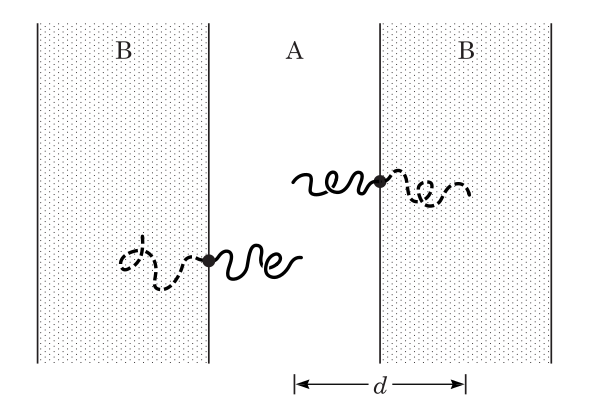
\includegraphics[scale=0.5]{./figures/FIG3-10.png}
	\caption{典型的$AB$型二嵌段共聚物在强分离层状中间相中的延伸链构象.当共聚物熔体的$A$,$B$嵌段高度不相容时,连接嵌段的连接点(固定点)强定位于$A$,$B$区域的界面.这些链还被垂直拉伸到界面外,达到典型的端到端距离$d$远远超过未扰动的$R_g$.}
	\label{FIG3.10}
\end{figure}

形如(\ref{FIG3.10}),在强隔离的嵌段共聚物中间相中也出现了类似情况.在二嵌段共聚物的$A$,$B$嵌段强烈不相容的条件下,相似链熔体中连接两嵌段的连接点强定位于不同区域间的界面.所以为了避免相互冲突并填满空间,单个的$A$,$B$块必须从界面扩展到各自富含$A$,$B$的域.

为了引入强拉伸近似,有必要回到势为$w(\mathbf{r})$的连续高斯链的路径积分描述.假设链的拉伸完全由电势决定.

描述聚合物链的统计权重的格林函数$g(\mathbf{r},\mathbf{r}',N;[w])$且$\mathbf{r}(0) = \mathbf{r}' \quad \mathbf{r}(N) = \mathbf{r}$可被写为:
\begin{equation}
g(\mathbf{r},\mathbf{r}',N;[w]) \propto \int_{\mathbf{r}(0) = \mathbf{r}'}^{\mathbf{r}(N) = \mathbf{r}}e^{-\beta U_0(\mathbf{r})-\beta U_1(\mathbf{r},w)}\,\mathcal{D}\mathbf{r}\label{3.188}
\end{equation}
其中忽略$g$的归一化.从而
\begin{equation}
Q[w] \propto \iint g(\mathbf{r},\mathbf{r}',N;[w])\,\mathrm{d}\mathbf{r}\mathrm{d}\mathbf{r}' \label{3.189}
\end{equation}

在聚合物满足端到端特征分离$|\mathbf{r}-\mathbf{r}'| \sim d$被强拉伸的情况下,式(\ref{3.188})中拉伸项$\beta U_0(\mathbf{r})$贡献的势能分布阶为$\epsilon^{-1} = \frac{d^2}{{R_g}^2}$其中$|\epsilon| \ll 1$.由于势能负责拉伸,$\beta$也必须为上述数量级.因此我们引入一个无量纲轮廓变量$t \in [0,1]$,以及无量纲聚合物形$\mathbf{x}(t)$:
\begin{equation}
t = \frac{s}{N},\qquad \mathbf{x}(t) = d^{-1}\mathbf{r}(s)
\end{equation}
定义按比例缩放的势能:
\begin{equation}
V(\mathbf{x}(t))\equiv \frac{{R_g}^2 N}{D^2}w(\mathbf{r}(s)) = \epsilon N w(\mathbf{r}(s))
\end{equation}
从而格林函数可被定义为
\begin{equation}
g(\mathbf{x},\mathbf{x}',1;[V]) \propto \int_{\mathbf{x}(0)=\mathbf{x}'}^{\mathbf{x}(1)=\mathbf{x}}e^{-\epsilon^{-1}\int_{0}^{1}[\frac{1}{4}(\frac{\mathrm{d}\mathbf{x}(t)}{\mathrm{d}t})^2+V(\mathbf{x}(t))]\,\mathrm{d}t}\,\mathcal{D}\mathbf{x} \label{3.192}
\end{equation}
其中$\epsilon^{-1} \gg 1$.

$\epsilon \rightarrow 0$时,对应于强拉伸链,这样的路径积分在缩放后的链结构$\mathbf{x}(t)$上可以用拉普拉斯方法渐近求值.强拉伸的首项阶的贡献因此起源于"经典"路径$\mathbf{x}^*(t)$,最大程度的减少"行动":
$$
S[\mathbf{x}] = \int_{0}^{1}[\frac{1}{4}(\frac{\mathrm{d}\mathbf{x}(t)}{\mathrm{d}t})^2+V(\mathbf{x}(t))]\,\mathrm{d}t 
$$
使得
\begin{equation}
g(\mathbf{x},\mathbf{x}',1;[V]) \sim e^{-\epsilon^{-1} S[\mathbf{x}^*]} \label{3.193}
\end{equation}

经典路径满足$Euler-Lagrange$方程:
\begin{equation}
\frac{1}{2}\frac{\mathrm{d}^2 \mathbf{x}^*(t)}{\mathrm{d}t^2} = \frac{\partial V(\mathbf{x}^*(t))}{\partial \mathbf{x}^*(t)} \label{3.194}
\end{equation}
其中边界条件为$\mathbf{x}^*(0) = \mathbf{x}'= \frac{\mathbf{r}'}{d},\quad \mathbf{x}^*(1) = \mathbf{x} = \frac{\mathbf{r}}{d}$.
"经典"指式(\ref{3.194})与经过势$U(\mathbf{x})= -V(\mathbf{x})$的粒子的牛顿力学的近似类比.将拉普拉斯方法系统地应用于$\epsilon$高阶方程,可以得到式(\ref{3.193})的高阶渐近修正.

对格林函数的经典或强拉伸近似的评估是通过求解给定势$w(\mathbf{r})$的式(\ref{3.194})和相关的边界条件来进行的.然后计算经典路径$\mathbf{x}^*(t),\, t\in [0,1]$的$S[\mathbf{x}]$
并通过(\ref{3.193})得到$g(\mathbf{r},\mathbf{r}',N;[w])$.对格林函数求值后,利用(\ref{3.189})对配分函数求近似,利用式$(3.50)$和式$(3.72)$对密度算子和对相关函数求近似.这种方法主要适用于电势足够简单的情况(如谐波),从而可以对(\ref{3.194})进行分析积分.如果求解经典运动方程需要数值方法,则强拉伸近似的实现比较繁琐,相对于$(3.22)$和$(3.25)$的直接数值计算几乎没有优势.




